\section{Domain Model}

Domain modellen bruges som en overgang mellem kravspecifikation og systemarkitektur. I kravspecifikation beskrives hvad der skal ske ved interaktion, mens systemarkitekturen beskrives hvordan systemet reagerer. Domain modellen bruges til at beskrive hele systemets domæne. Her kigges ikke på hardware vs. software, der kigges i stedet på "enheder" og deres ansvarsområder.

På figur \ref{fig:domain_model} vises domain model tilhørende systemet. De fire øverste enheder i domain modellen dækker over ansvarsområder som har men systemets webapplikationen at gøre. De resterende enheder er alle tilknyttet ansvarsområder der har med dronen at gøre.

På domain modellen vises at bruger kommunikerer med dronen gennem en website. Websiden har forbindelse til en server som kan sende instruktioner videre til arduino'en. Det vises at kommunikation mellem server og arduino går gennem 3G netværket. Under flyvning kontrollerer arduino kamera, afstandssensorer og quadrocopter. 

\vspace{-5pt}
%kommentar
\begin{figure}[H]
	\centering
	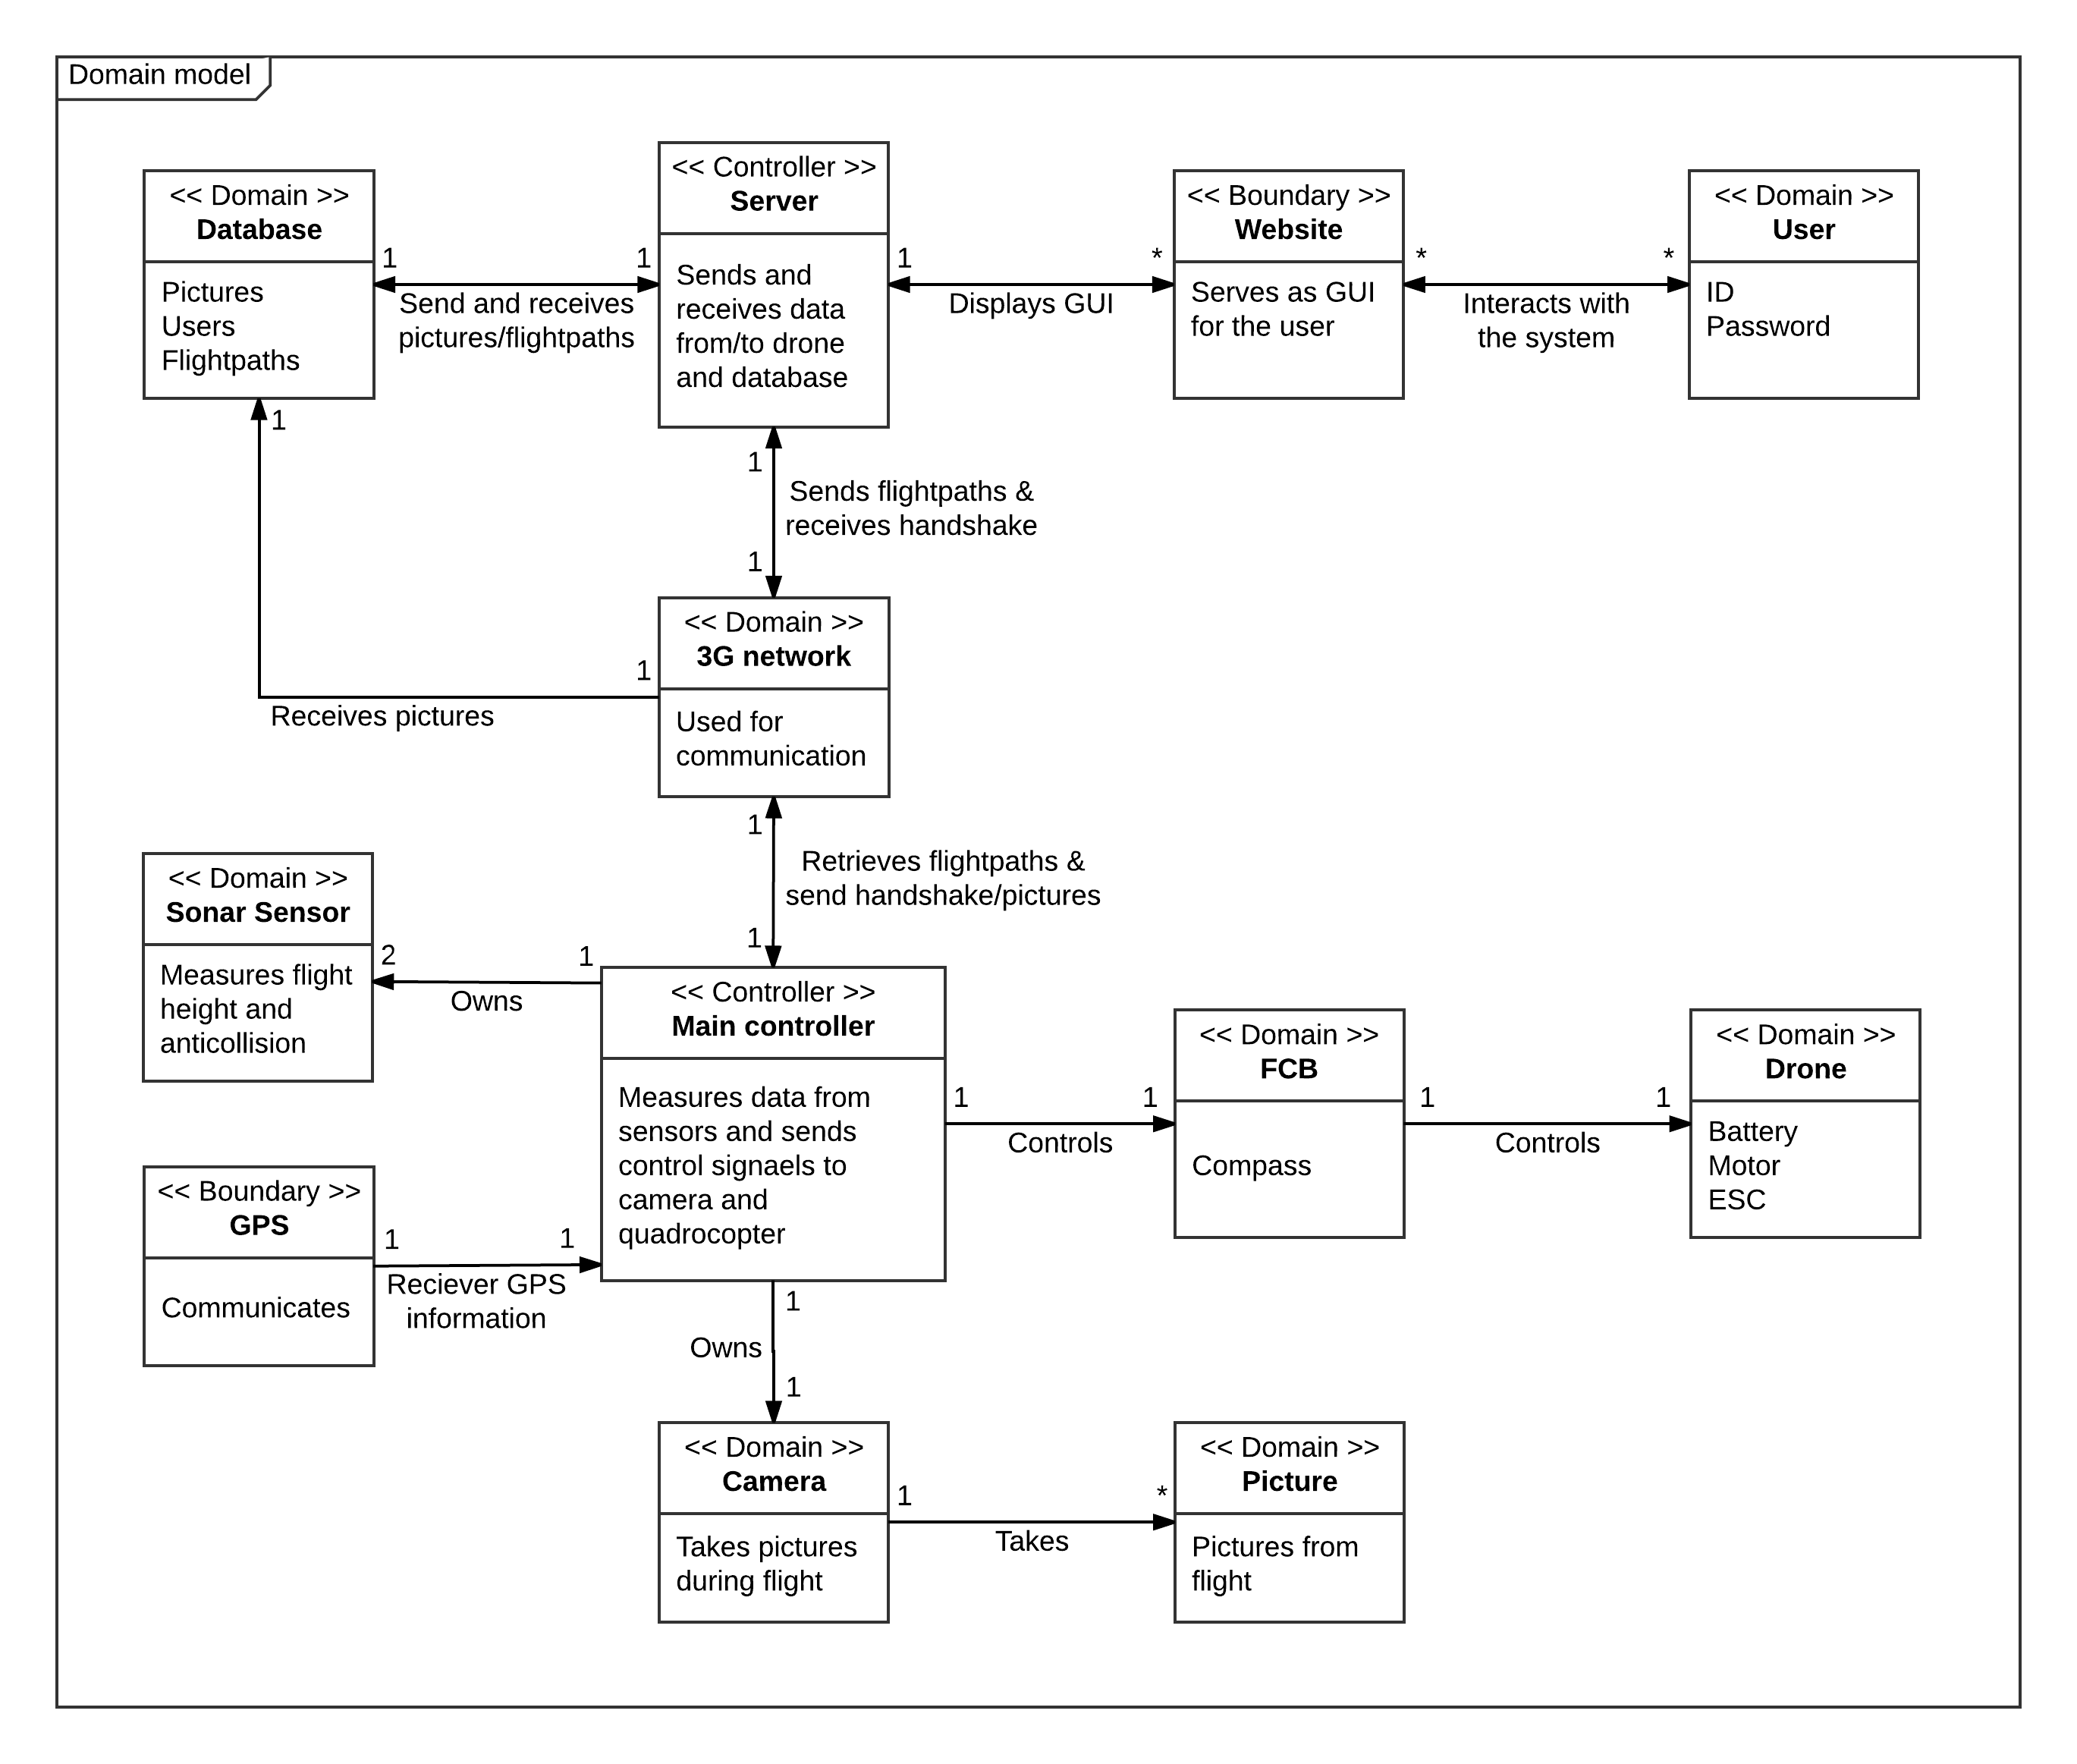
\includegraphics[width=1.\textwidth]{Billeder/domain_model.png}
	\vspace{-5pt}
	\caption{Domain model}
	\label{fig:domain_model}
\end{figure}